\documentclass{beamer}
\usepackage[export]{adjustbox}
\usepackage{svg}

%\usetheme{lucid}
\begin{document}
\frame{
	\frametitle{SBI for EEG-data}
	\framesubtitle{}
	Scheme: Combining posterior of first subset with prior of next subset
\begin{figure}
\label{fig:scheme}
  \centering

  \includesvg[width=10cm, inkscapelatex=false]{images/scheme.svg}
  \caption{\label{figure:scheme}\textbf{Neural Incremental Posterior Estimation.}\small .}

\end{figure}
	
	
		
	}
	
	
\frame{
	\frametitle{Method}
	- $\Theta_1, \Theta_2, \Theta_3$ are parameter subsets\\
	- $x_1, x_2, x_3$ are summary statistic subsets \\
	\vspace{5pt}
	
	We approximate $p(\Theta_1, \Theta_2, \Theta_3| x_1, x_2, x_3)$ by incrementally increasing the number of inferred parameters\\
	\vspace{7pt}
	
	1.) We reduce $p(\Theta_1|x_1, x_2, x_3)$ to $p(\Theta_1|x_1)$ by making the assumption that $x_1$ has the highest impact on $\Theta_1$. Approx. by neural net: $\hat{p}(\Theta_1|x_o) = q_{F(x_o,\phi)}(\Theta_1)$\\
	\vspace{5pt}
	2.) We learn $p(\Theta_1, \Theta_2|x_1, x_2)$ by using the combined proposal: $ \Tilde{p} = p(\Theta_1|x_1) \cdot p(\Theta_2)$, assuming independent priors. Approx. by neural net: $\hat{p}(\Theta_1, \Theta_2|x_o) = q_{F(x_o,\phi)}(\Theta_1, \Theta_2)$\\
	\vspace{5pt}
	3.) further subsets...



}

	
	\frame{
		\frametitle{Gaussian toy example}
		\framesubtitle{}
\begin{figure}
 \centering
    \begin{minipage}[h]{13cm}
        \small (a)  \hspace{6cm}  (b)  
    \end{minipage}
        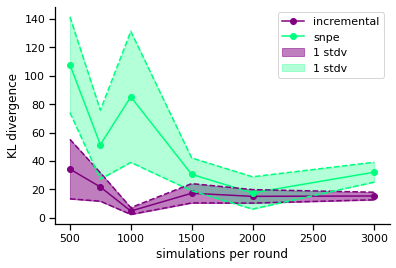
\includegraphics[width=0.42\linewidth]{images/thesis_fig4_3a.png}
        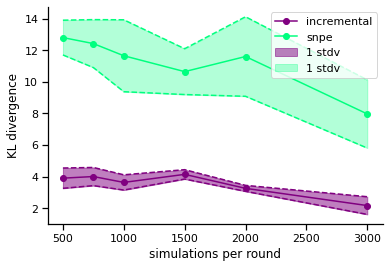
\includegraphics[width=0.42\linewidth]{images/thesis_fig4_3b.png}
        %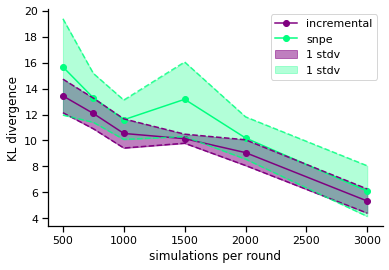
\includegraphics[width=0.31\linewidth]{images/thesis_fig4_3c.png}

        
\caption{\label{kldiv2}\textbf{KL divergence} (a) mdn (b) maf  }

\end{figure}

		
	}	



	\frame{
	\frametitle{Over-dispersion of last subset}
	\framesubtitle{}
\begin{figure}[h]
 \centering

        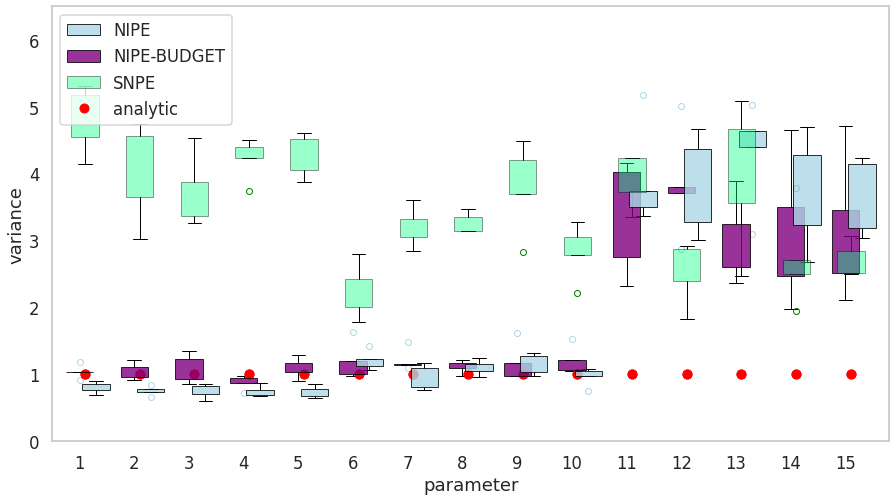
\includegraphics[width=0.8\linewidth]{images/toy_example_maf_03_05_ratio.png}
        
        
\caption{\label{boxplot}\textbf{Box plot for the variances of inferred and analytic posteriors}. }

\end{figure}
	

}

	\frame{
	\frametitle{ERP - Posterior predictive check of two experimental conditions}
	\framesubtitle{}
	
 \begin{figure}[!ht]
 \centering


        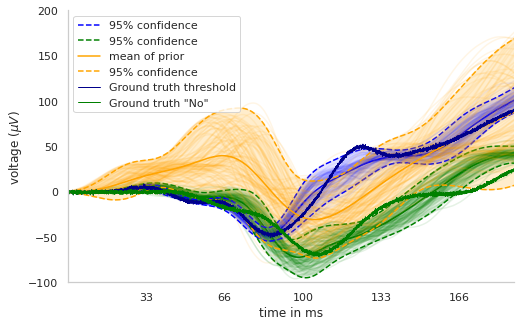
\includegraphics[width=0.70\linewidth]{images/ppc_threshold_versus_No_nipe.png}


\caption{\label{exp_ppc}\textbf{PPC - derived with NIPE (nsf)} \small The simulations drawn from the prior are visualized in orange (95\% confidence intervals), while simulations from the threshold samples are visualized in blue and simulations from the 'No' samples are visualized in green. }

\end{figure}
	 

}

\frame{
	%\frametitle{Contour comparison}
	\framesubtitle{}

 \begin{figure}[!ht]
 \centering


        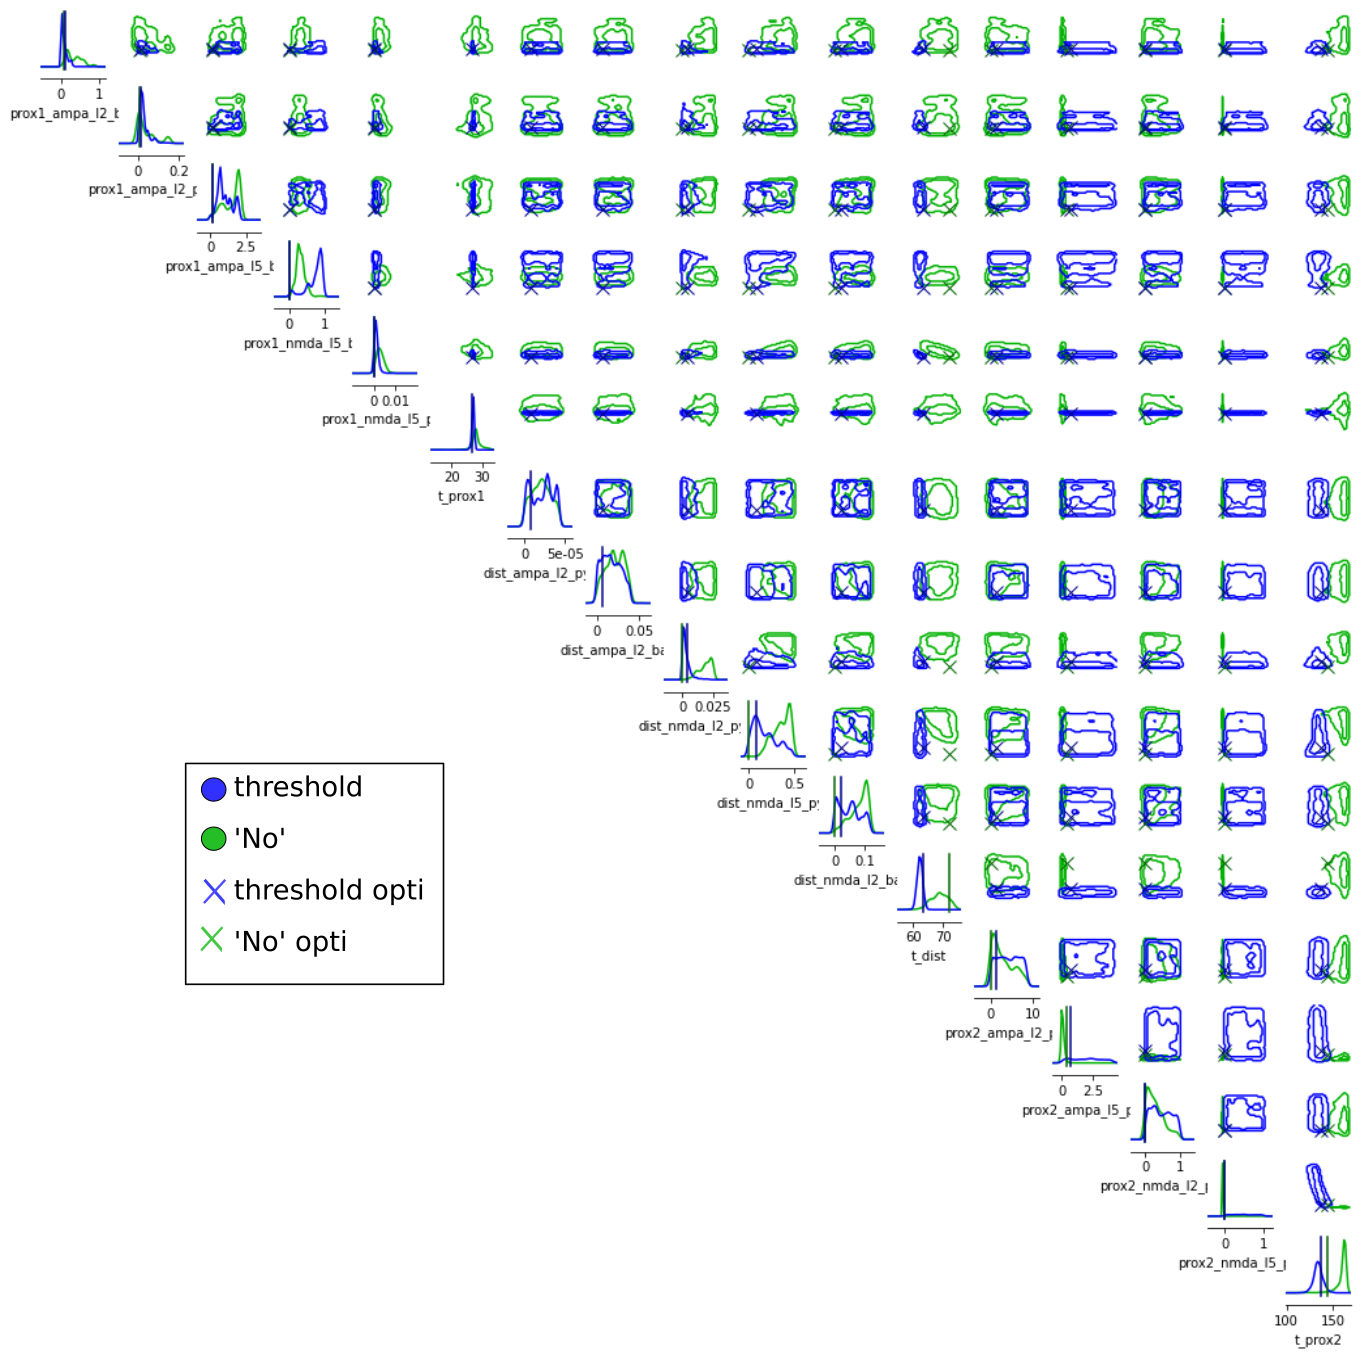
\includegraphics[width=0.90\linewidth]{images/contour_plots_threshold_versus_no_green_blue4.png}
        


\caption{\label{contour_opti}\textbf{Density plot - Comparison to Optimization tutorial} \small (a) shows the 1d (diagonal) and 2d marginals (off-diagonal) for the threshold condition, derived with NIPE. The dark green crosses and lines indicate the optimized values of the 'No' condition from the tutorial, while the dark blue crosses/lines indicate the same for the threshold condition.}

\end{figure}


}


\frame{
	\frametitle{Stochasticity and flexibility of model}
\centering

	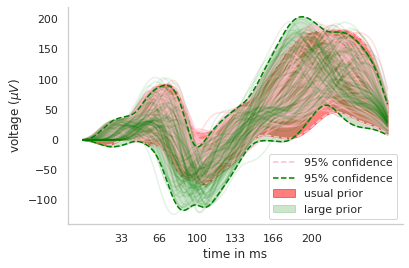
\includegraphics[height=4cm]{images/ppy_large_versus_small_prior.png}
	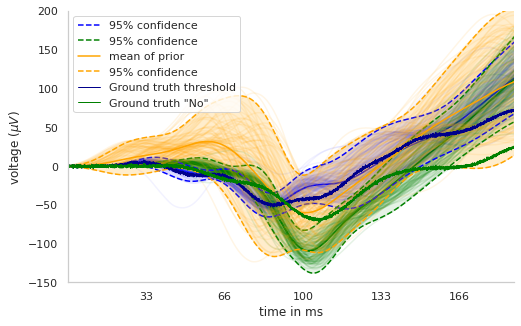
\includegraphics[height=4cm]{images/ppc_threshold_largeprior_versus_No_largeprior_nipe.png}
}

\frame{
	\frametitle{Difficulties/Questions}
	\begin{itemize}
	\item[--] last subset probably not well restricted
	\item[--] how to choose good priors that fit all conditions?
	\item[--] leakage correction / importance weights - SNPE sometimes has a low acceptance rate.. sampling takes long. We do not have this problem for NIPE
    \item[--] Including standard deviation is done by Jones, but does not seem 'scientifically smooth'
	\end{itemize}



}


\frame{
	\frametitle{Further results}

 \begin{figure}
 \centering

        \small \textbf{(a)}
        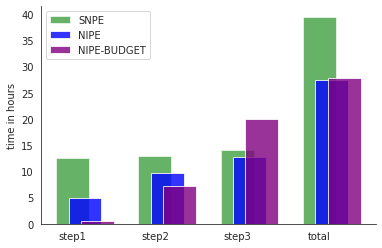
\includegraphics[width=0.41\linewidth]{images/thesis_fig4_9_time.png}
        \small \textbf{(b)}
        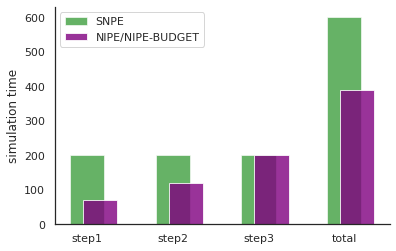
\includegraphics[width=0.41\linewidth]{images/thesis_fig4_9_simtime.png}



\caption{\label{time}\textbf{Time for each step - comparison between SNPE and NIPE} \small }

\end{figure}
}

\frame{
	%\frametitle{Further results}

	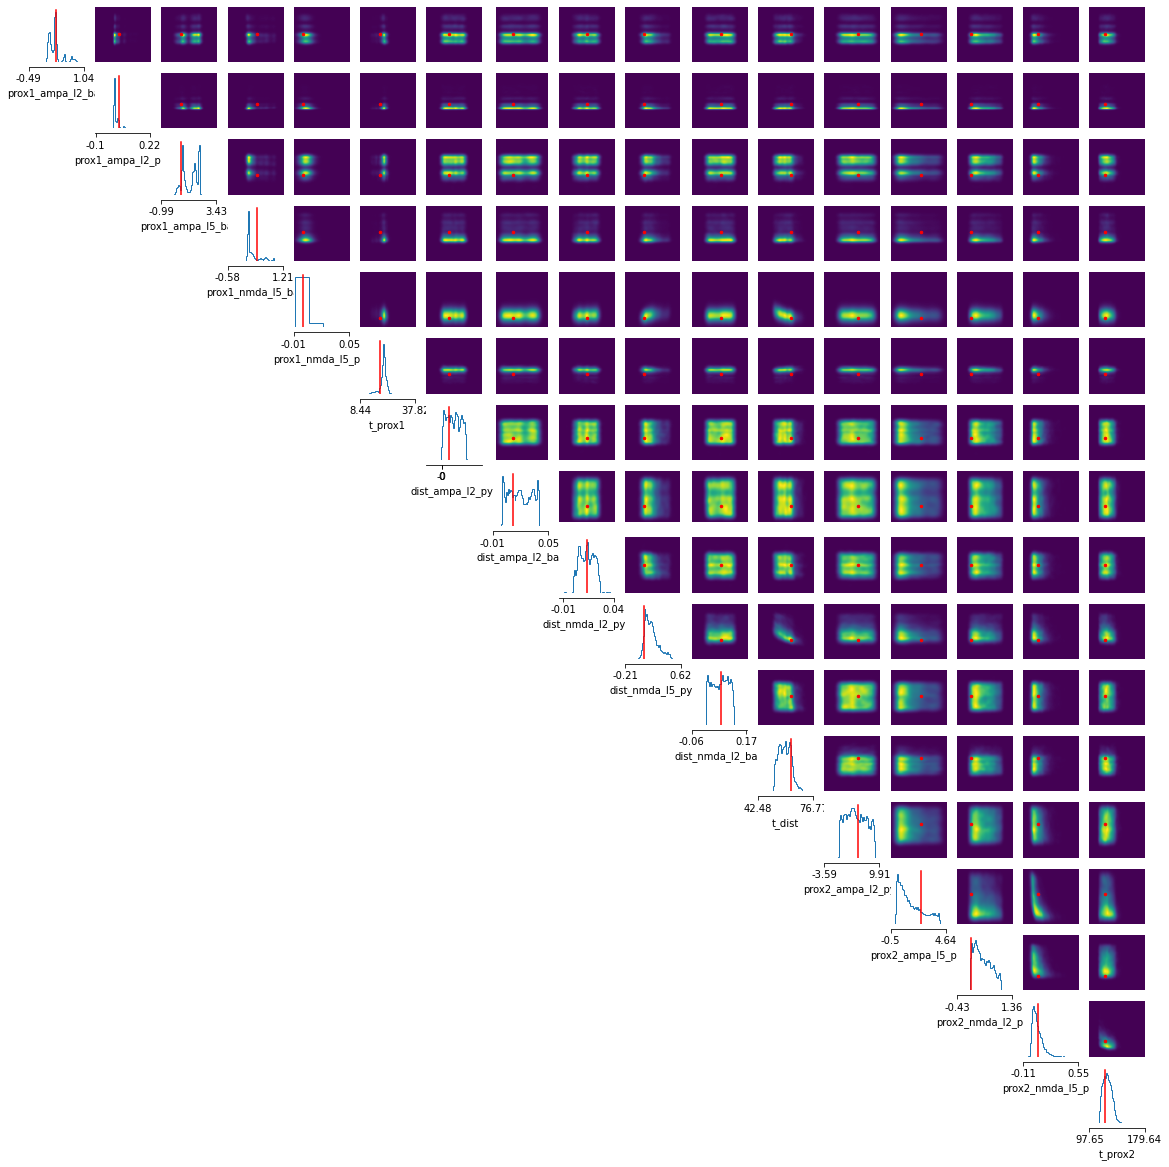
\includegraphics[width=0.92\linewidth]{images/kde_normal4.png}
}



\frame{
	\frametitle{Further results}

        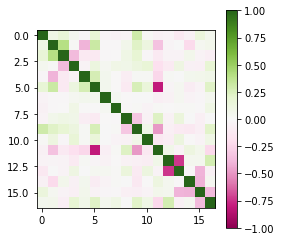
\includegraphics[width=0.4\linewidth]{images/thesis_fig4_8b.png}
        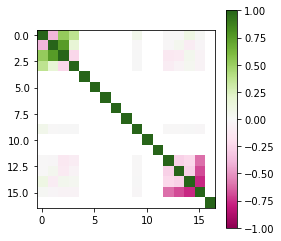
\includegraphics[width=0.4\linewidth]{images/thesis_fig4_8c.png}
}



\end{document}